\documentclass[a4paper,12pt]{scrreprt}
    %% Used for changing geometry of the page
    %% Cover page text cannot overlay cover sketching/style
    %% https://ctan.org/pkg/geometry?lang=en
\usepackage{geometry}
    %% Changes language of some packages protocols
    %% e.g., when captioning images: Figure 1. -> Figura 1.
    %% https://ctan.org/pkg/babel?lang=en
\usepackage[portuguese]{babel}
    %% Used for special fonts
    %% Cannot be compiled with pdflatex
    %% https://ctan.org/pkg/fontspec?lang=en
\usepackage{fontspec}
    %% Arial FONT
    \setmainfont{Arial}
    %% More colors and color options
    %% https://ctan.org/pkg/xcolor?lang=en
    %% https://ctan.org/pkg/colortbl?lang=en
\usepackage{xcolor,colortbl}
    %% More tabular options, like dashed/dotted lines
    %% https://ctan.org/pkg/arydshln?lang=en
\usepackage{arydshln}
    %% List of acronyms
    %% https://ctan.org/pkg/nomencl?lang=en
\usepackage[intoc]{nomencl}
    %% Must be called to init nomencl environment
    \makenomenclature
    %% More images options/settings
    %% https://ctan.org/pkg/graphicx?lang=en
\usepackage{graphics}
    %% Defining subdirectories to image path enviornment
    %% \graphicspath{{sub1}{sub2}...{subN}}
    \graphicspath{{images}}

    %% used to handle cross-referencing commands in LaTeX to produce hypertext links in the document
    %% https://ctan.org/pkg/hyperref?lang=en
\usepackage{hyperref}
    %% math environments
    %% https://ctan.org/pkg/amsmath?lang=en
    %% settings
    \hypersetup{
        colorlinks,
        citecolor=black,
        filecolor=black,
        linkcolor=black,
        urlcolor=black
    }

\usepackage{amsmath}
    %% Defining backgrouns, used to make the cover
    %% https://ctan.org/pkg/background?lang=en
\usepackage[some]{background}
    %% Used to make drawings or complex graphics
    %% http://pgf.sourceforge.net/pgf_CVS.pdf
\usepackage{tikz}
    %% Tikz library to point operations ((x1,y1) + (x2,y2))
    \usetikzlibrary{calc}

%% code snippets
\usepackage{listings}
\usepackage{color}

\lstset{
    frame=tb,
    language=SQL,
    aboveskip=3mm,
    belowskip=3mm,
    showstringspaces=false,
    columns=flexible,
    basicstyle={\small\ttfamily},
    numbers=left,
    numberstyle=\small\color{gray},
    keywordstyle=\color{blue},
    commentstyle=\color{dkgreen},
    stringstyle=\color{mauve},
    breaklines=true,
    breakatwhitespace=true,
    tabsize=3,
    moredelim=**[is][\color{blue}]{@}{@}
}

%% Defining sfdefault font and default font for document
\renewcommand{\familydefault}{\sfdefault}

%% For tables
\usepackage{pbox}
\usepackage{longtable}
\usepackage{xcolor} % for coloring rows
\usepackage{multirow}
\usepackage{hhline}
\usepackage{array}

% Custom ColumnSpec for tables
\newcommand{\MyColumnSpec}{|p{0.3cm}|p{4cm}|p{3cm}|p{4.5cm}|p{3cm}|}

%% changing chapter and section title style and spacing
\usepackage{titlesec}
\titleformat{\chapter}[hang]%
  {\sffamily\Huge\bfseries}% format applied to label+text
  {\thechapter}%% label
  {0.5em}% horizontal separation between label and title body
  {}% before the title body
  []% after the title body

\titleformat{\section}[hang]%
  {\sffamily\Large\bfseries}% format applied to label+text
  {\thesection}%% label
  {0.5em}% horizontal separation between label and title body
  {}% before the title body
  []% after the title body

\titlespacing*{\chapter}{0pt}{*0}{*0}
\titlespacing*{\section}{0pt}{*0}{*0}

% Paragraph vertical spacing
% \usepackage{parskip}
% \setlength{\parskip}{5pt}

%==========================================================================
% DOCUMENT
%==========================================================================

\begin{document}

\pagenumbering{gobble}

%% Costume made cover
%% From there you can use \makecover command to build the cover
%% Orange cover color
\definecolor{titlepagecolor}{RGB}{47,113,187}

%==========================================================================
% COLORED BAR ON THE LEFT SIDE
%==========================================================================

\backgroundsetup{
    scale=1,
    angle=0,
    opacity=1,
    contents={
        \begin{tikzpicture}[remember picture,overlay]
            \path [fill=titlepagecolor] (-10.5,-15) rectangle ++ (5,30);
            \node[color=white] at (-7.2,-12) {\bfseries {\fontsize{120}{60} \textsf{D}}};
            \node[color=titlepagecolor] at (-4.3,-12) {\bfseries {\fontsize{120}{60} \textsf{S}}};
            \node[color=titlepagecolor] at (-2,-12) {\bfseries {\fontsize{120}{60} \textsf{S}}};
        \end{tikzpicture}
    }
}

%==========================================================================
% TITLE PAGE INFO
%==========================================================================

%% Changes values in this field to show information in the cover and back cover about your team/project

%% TITLE
\title{\LARGE{Aplicação de Gestão de Turnos}}

%% AUTHORS
\author{
    Afonso Dionísio Santos (A104276) \\
  \quad
    Afonso Gonçalves Pedreira (A104537) \\
  \quad
    Dário Silva Guimarães (A104344) \\
  \quad
    Flávia Alexandra Silva Araújo (A96587) \\
  \quad
    Miguel Torres Carvalho (A95485)
}

%% Date

\date{\today}

%% Course
\newcommand{\Course}{Licenciatura em Engenharia Informática}

%% Department
\newcommand{\Department}{Escola de Engenharia}

%% UniName
\newcommand{\UniName}{Universidade do Minho}

%% UniPic
\newcommand{\UniPic}{
\includegraphics[width=120pt]{images/eeum.png}}

%% University
\newcommand{\University}{
    \begin{flushleft}
        \UniPic
    \end{flushleft}
    \textcolor{gray}{\small\textbf{\textsf{\UniName}}}\par
    \textcolor{gray!80!white}{\small{\textsf{\Department}}}\par
    \textcolor{gray!70!white}{\small{\textsf{\Course}}}
}

%% UC
\newcommand{\UC}{
    \begin{flushleft}
        \par\textcolor{titlepagecolor}{\Large\textbf{\textsf{Desenvolvimento de Sistemas de Software}}}
    \end{flushleft}
}

%% Project Phase
\newcommand{\ProjectPhase}{
    \begin{flushleft}
        \large\textbf{Trabalho Prático - Fase 3}
    \end{flushleft}
}

%% Group Info
\newcommand{\GroupInfo}{\par Grupo 14}

%% GitHub Repo
\newcommand{\GitHubRepo}{\par\url{https://github.com/LEI-DSS/DSS2425-Grupo-14}}

%% School Year
\newcommand{\SchoolYear}{
    \par\small{\textsf{Ano Letivo de 2024/2025}}
}

%% Define new command to show title, author and date
\makeatletter
\let\Title\@title
\let\Author\@author
\let\Date\@date
\makeatother

%==========================================================================
% BEGIN COVER PAGE
%==========================================================================

% Make cover page
\newcommand{\makecover}{

%% Removes page number on footer
\thispagestyle{empty}

%% No indentation
\setlength{\parindent}{0em}

%% Put Background defined on \backgroundsetup, in this page
\BgThispage

%% Changing geometry to prevent overlay with text
%% At the end of back cover, geometry is default with \restoregeometry
\newgeometry{top=4cm,left=6cm,right=2cm,bottom=2cm}

%% builds university info defined previously
\University
\vspace{1cm}
\UC
\ProjectPhase
\GroupInfo
\GitHubRepo
\vspace{0.5cm}
\SchoolYear

\vspace*{4cm}
%% bigger space (i think its the default one) between paragraphs
\setlength{\parskip}{1em}

%% builds title info defined previously
\par\textbf{\textsf{\huge\Title}}
\vspace{1cm}
%% builds author(s) info defined previously
\par\Author

\vspace{0.5cm}

%% builds date info defined previously
\par\Date
\restoregeometry
\pagebreak

%==========================================================================
% END COVER PAGE
%==========================================================================
}


% builds the cover
\makecover

%% smaller footer and header size
\newgeometry{top=2cm,left=3cm,right=3cm,bottom=3.5cm}
\savegeometry{default}

%==========================================================================
% BEGIN ABSTRACT PAGE
%==========================================================================

%% Abstract name: \Large font size, flushed left and paragraph skip before abstract content
% \renewenvironment{abstract}
%  {\par\noindent\textbf{\Large\abstractname}\par\bigskip}
%  {}
%
% \begin{flushleft}
% \begin{abstract}
%     Exemplo
%
%     \textbf{Área de Aplicação}: Exemplo
%
%     \textbf{Palavras-Chave}: Exemplo
%
% \end{abstract}
% \end{flushleft}
%
% \pagebreak

%==========================================================================
% END ABSTRACT PAGE
%==========================================================================

%==========================================================================
% BEGIN INDEXES PAGES
%==========================================================================

%% Changes table of content name
\renewcommand{\contentsname}{Índice}
\renewcommand{\listfigurename}{Índice de Figuras}
\renewcommand{\listtablename}{Índice de Tabelas}

\tableofcontents

\pagebreak

% \listoffigures
%
% \pagebreak

% \listoftables
%
% \pagebreak

%==========================================================================
% END INDEXES PAGES
%==========================================================================

%==========================================================================
% BEGIN MODELO DE ANÁLISE
%==========================================================================

%% Starting page numbering here
\pagenumbering{arabic}

\chapter{Modelo de Análise}
\vspace{2cm}

\begin{minipage}{\textwidth}
    \centering
    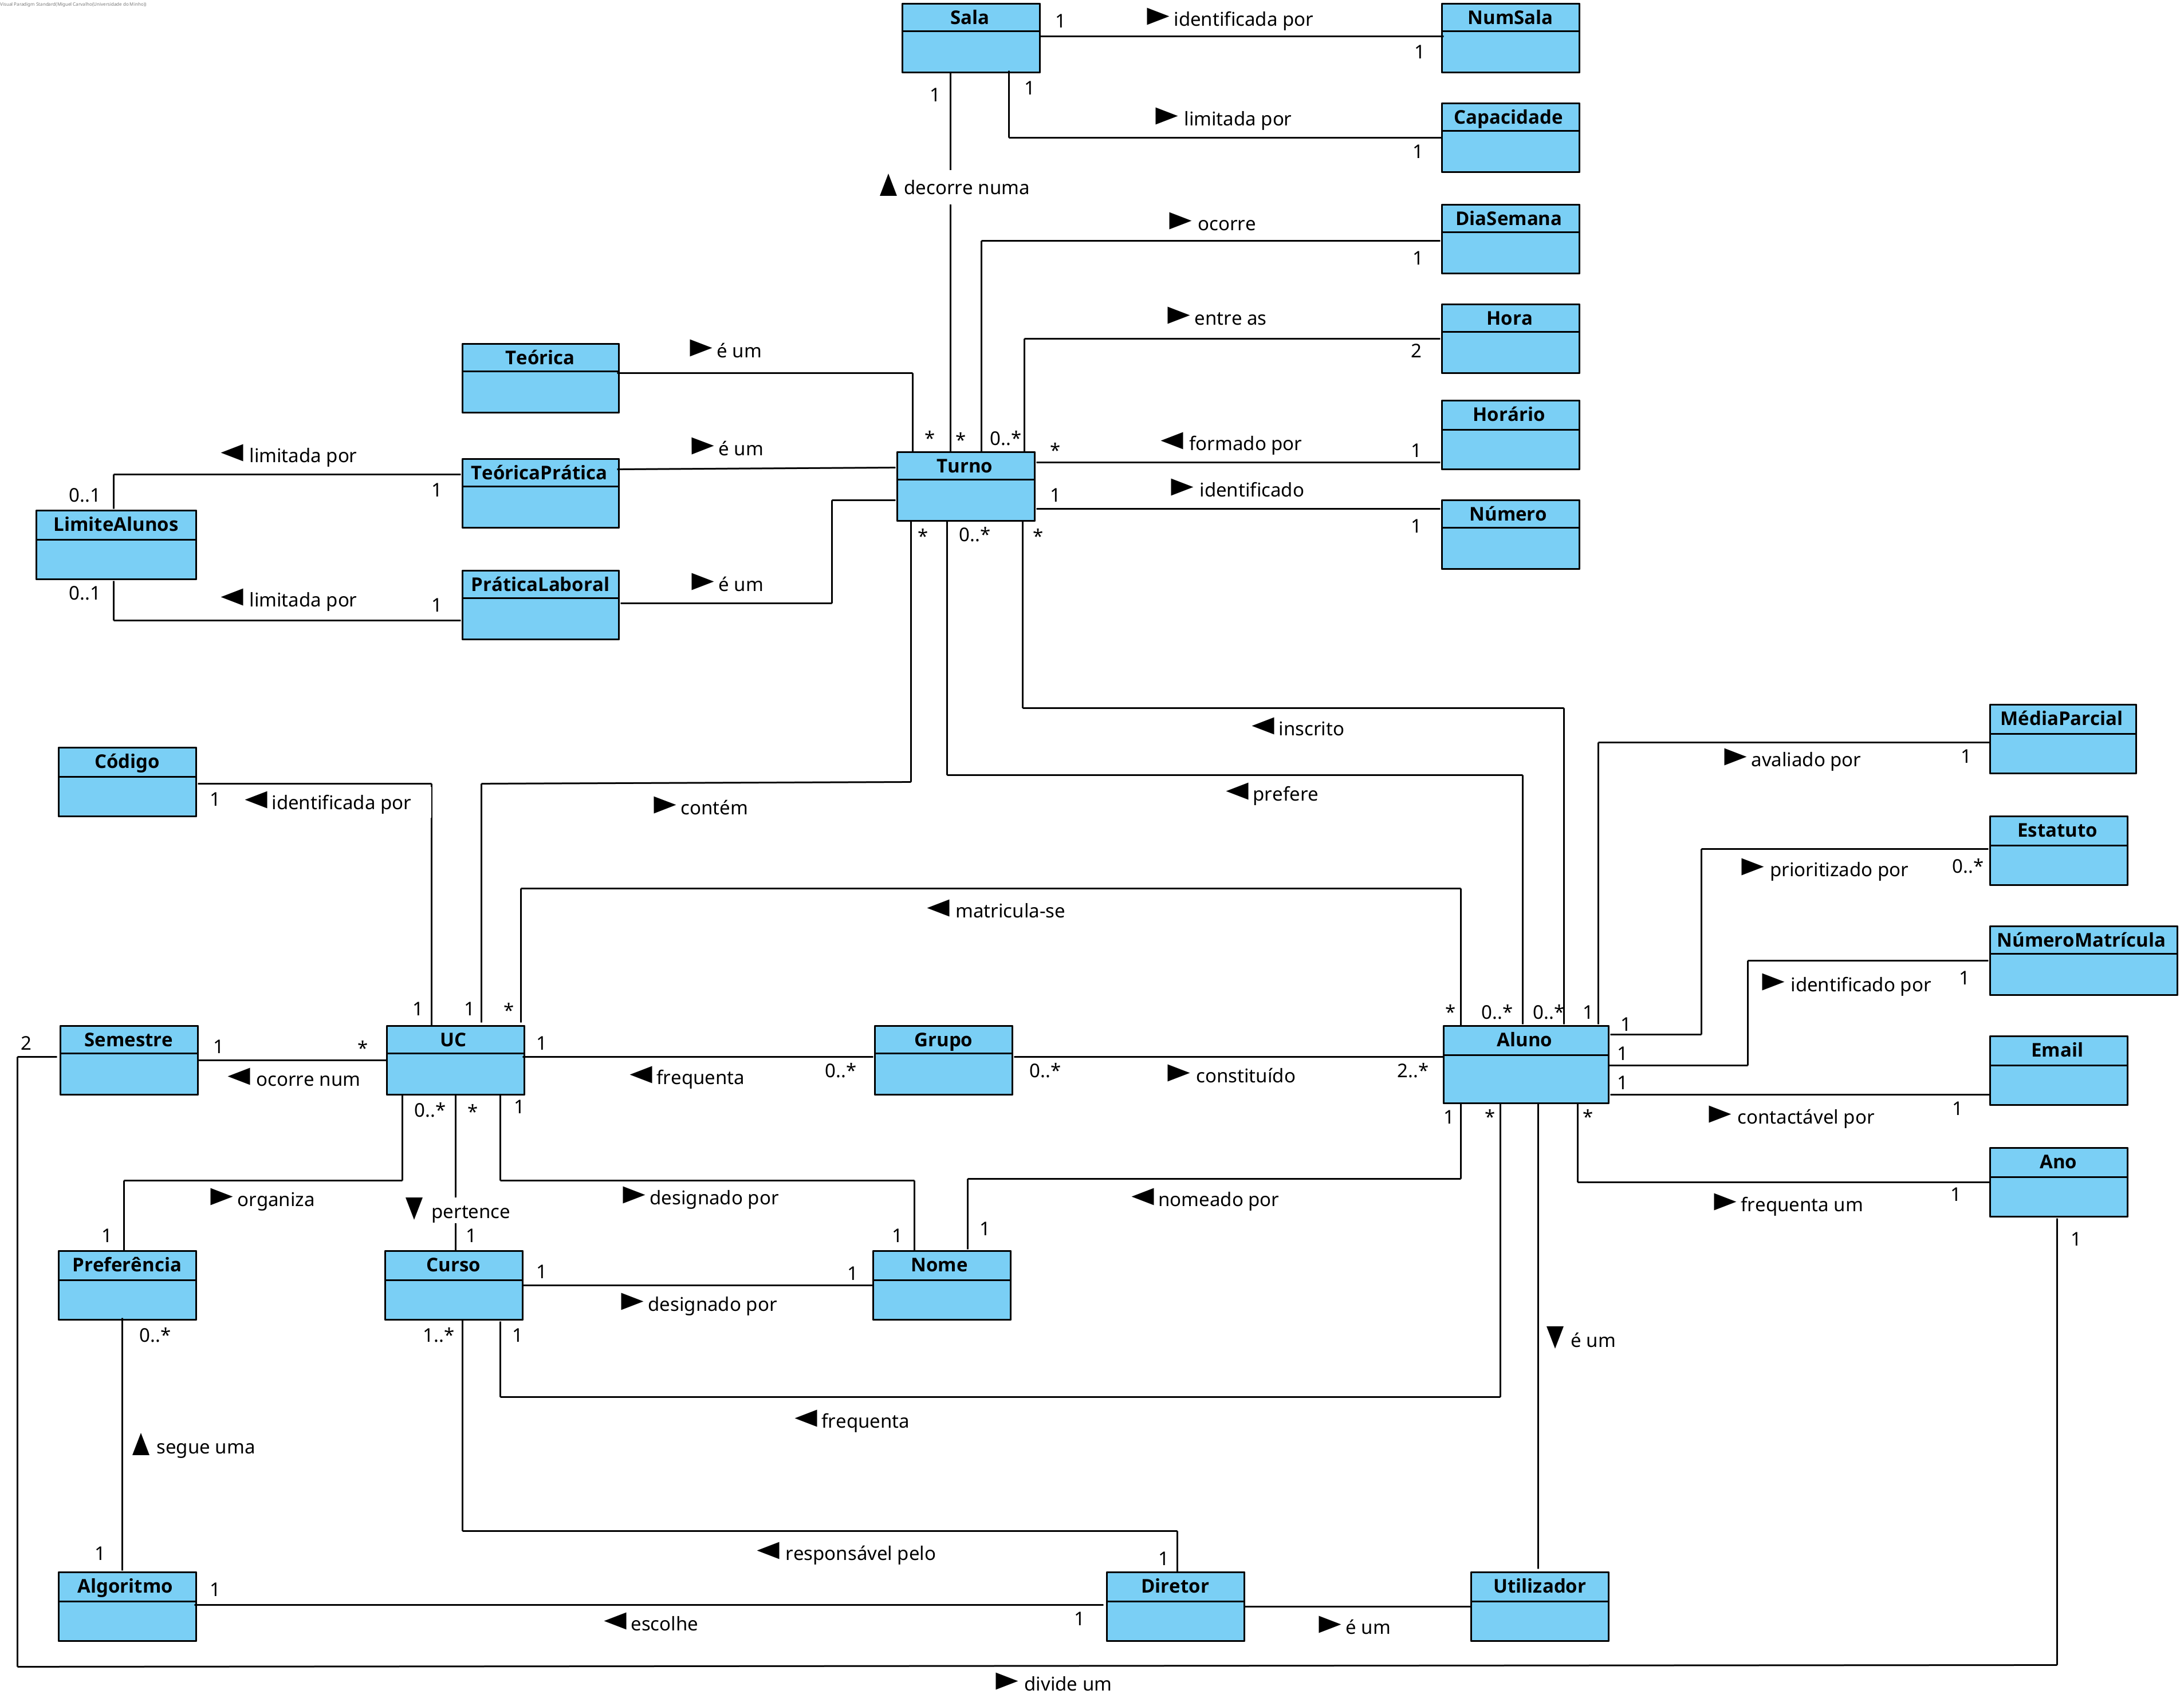
\includegraphics[width=1\textwidth]{images/modelo-analise.png}
    \captionof{figure}{Modelo de Análise}
    \label{fig:modelo_analise}
\end{minipage}

%==========================================================================
% END MODELO DE ANÁLISE
%==========================================================================

%==========================================================================
% BEGIN DIAGRAMAS DE CASOS DE USO
%==========================================================================

\chapter{Diagramas de Casos de Uso}
\vspace{1cm}

\begin{minipage}{\textwidth}
    \centering
    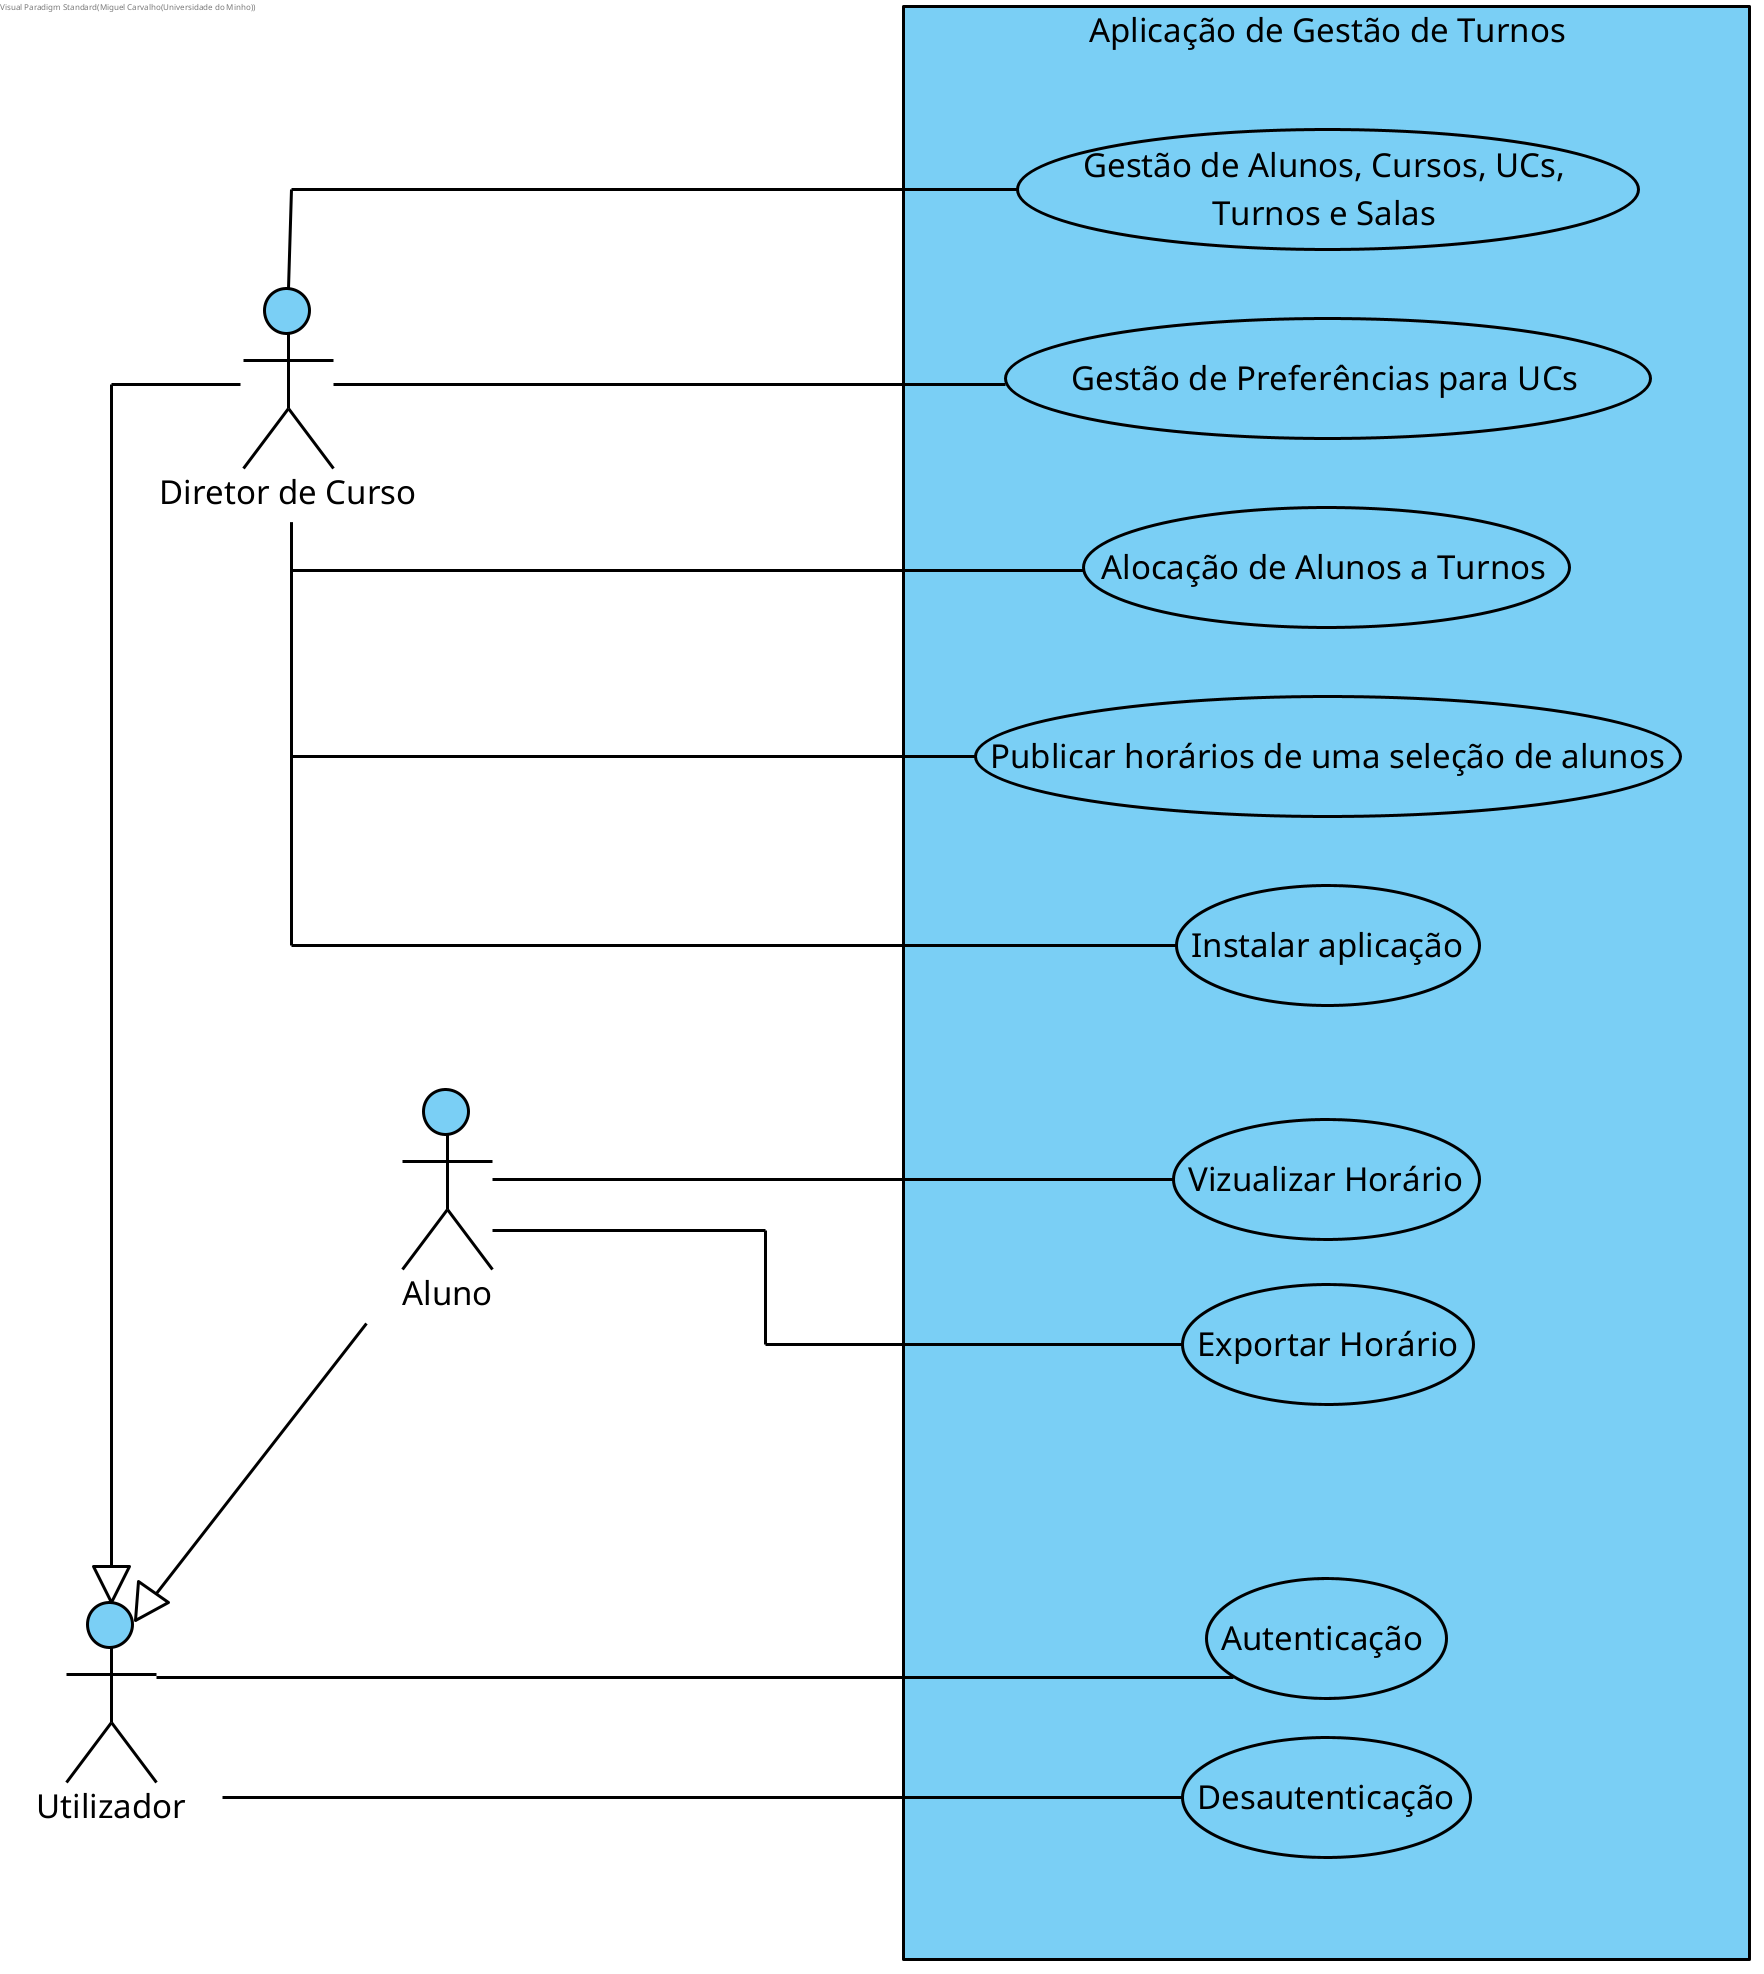
\includegraphics[width=1\textwidth]{images/use-cases/diagrams/1-geral.png}
    \captionof{figure}{Diagrama de Casos de Uso - Geral}
    \label{fig:2-1-diagrama_de_casos_de_uso_geral}
\end{minipage}

\begin{minipage}{\textwidth}
    \centering
    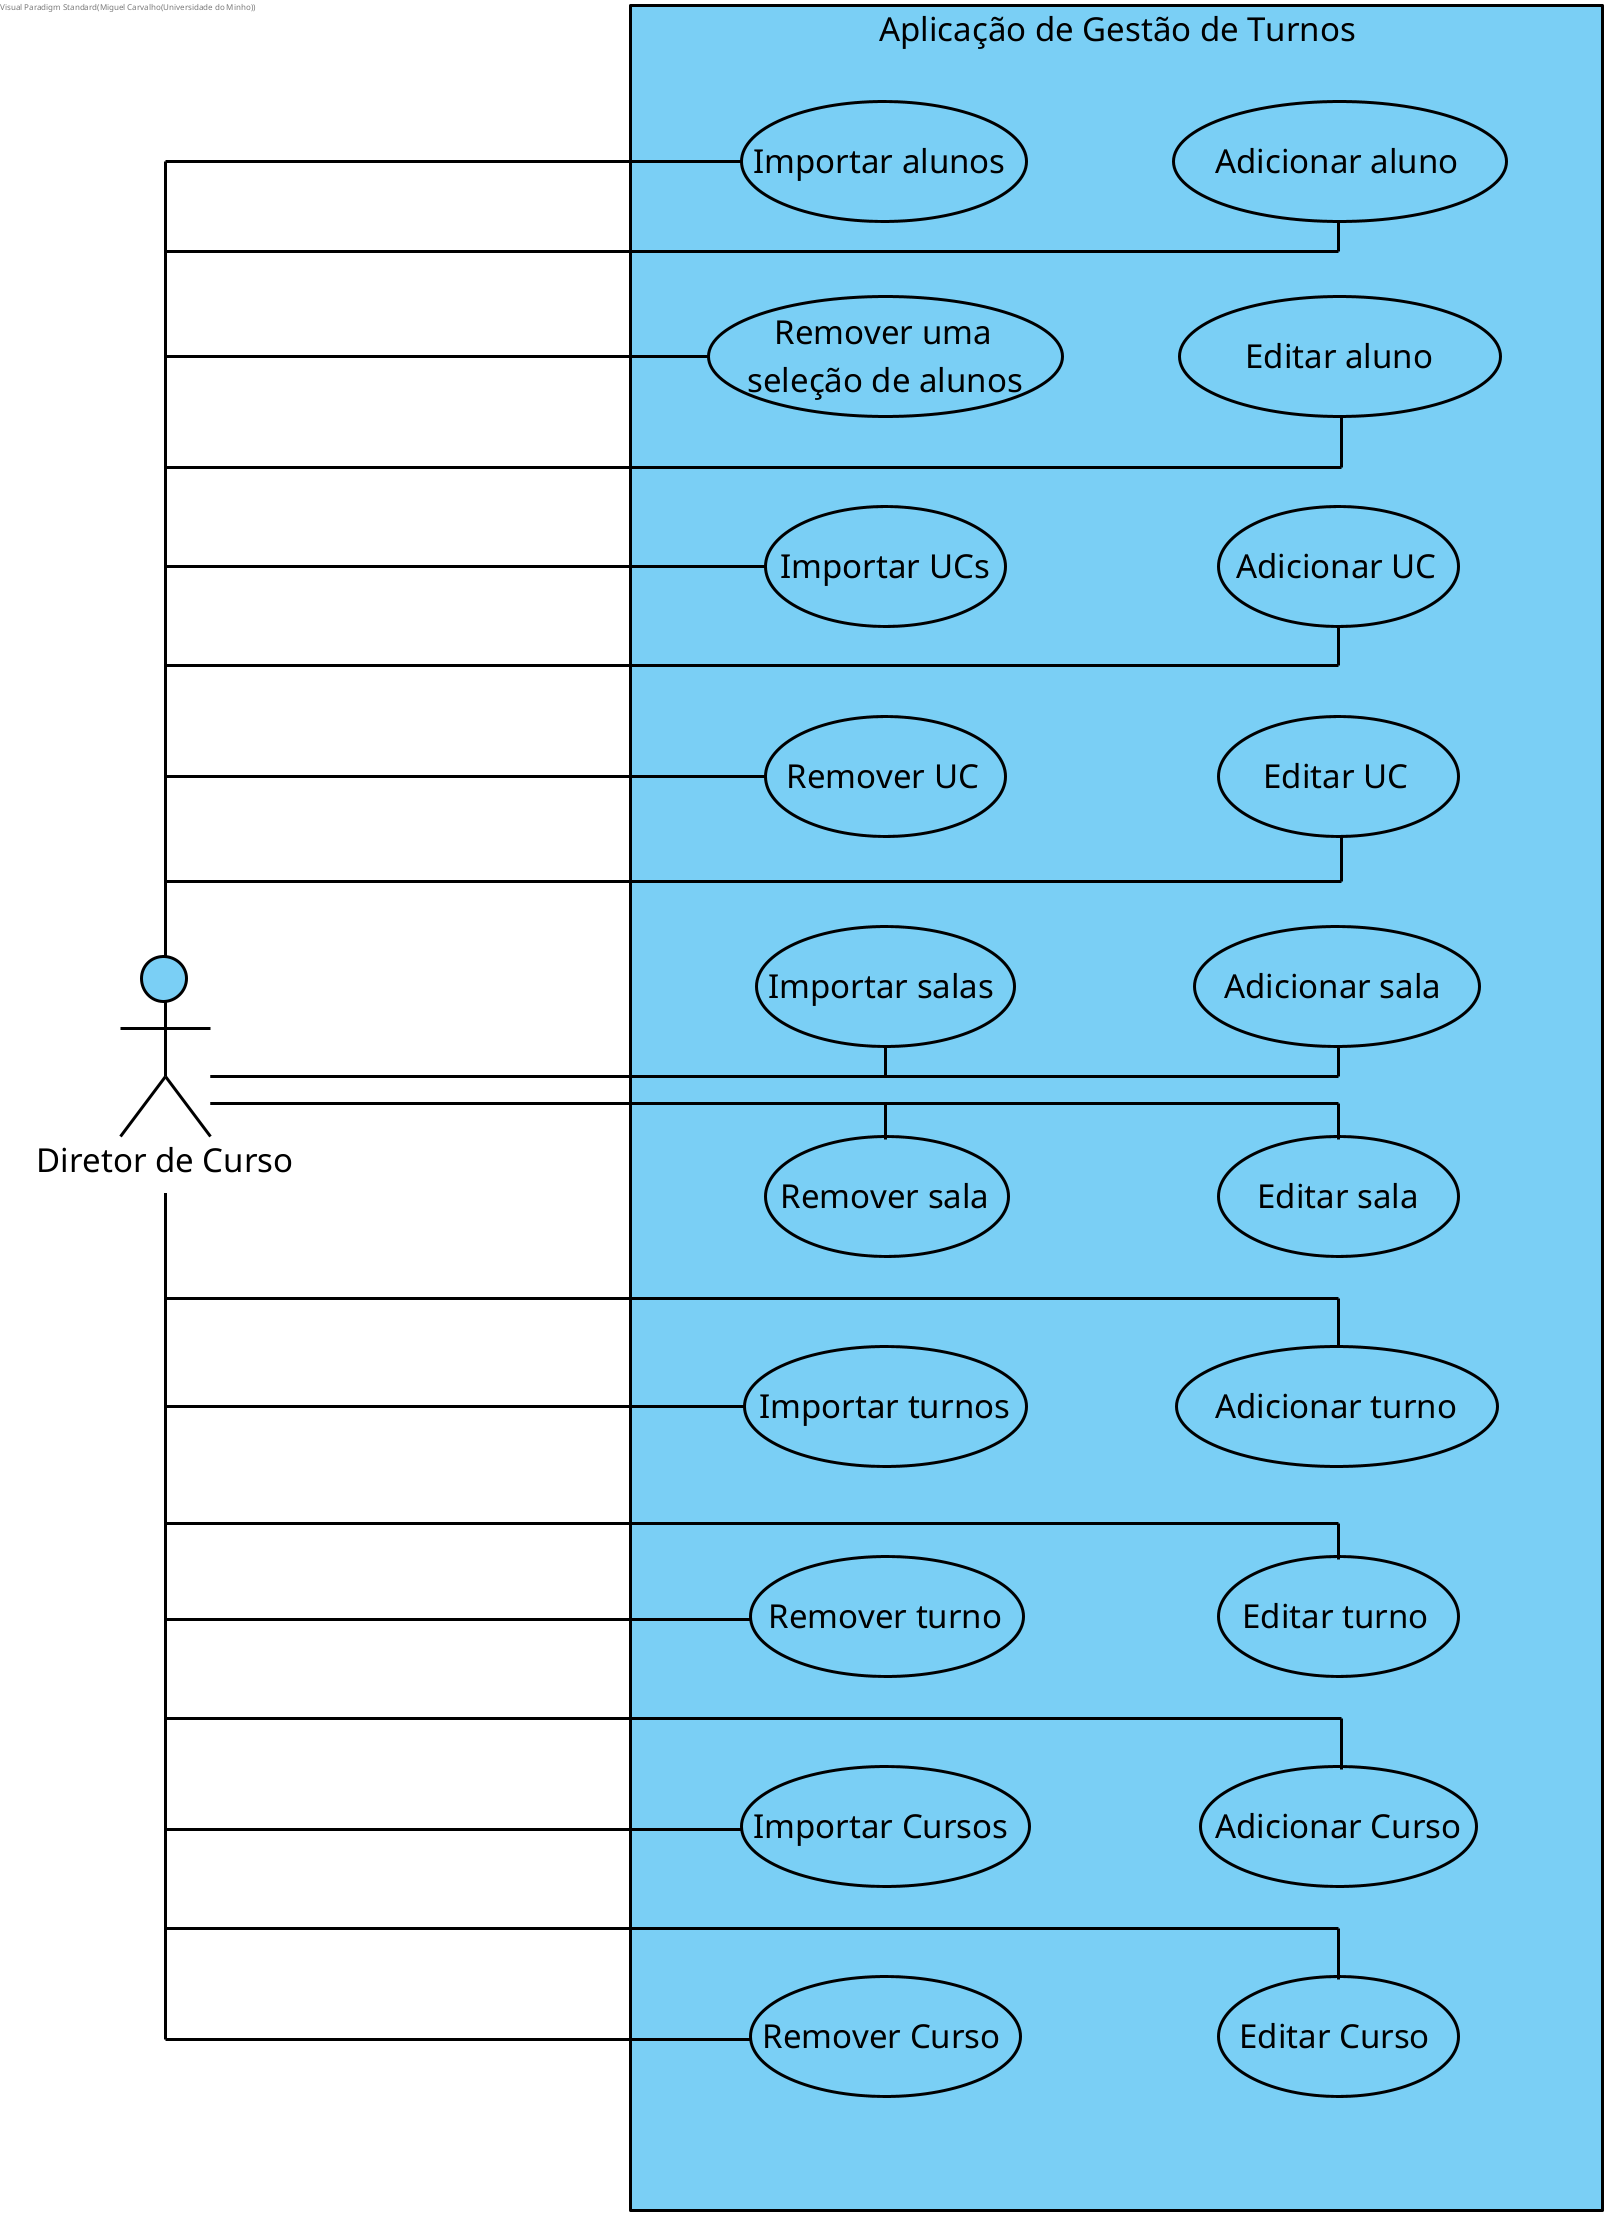
\includegraphics[width=1\textwidth]{images/use-cases/diagrams/2-gestao-alunos-cursos-ucs-turnos-salas.png}
    \captionof{figure}{Diagrama de Casos de Uso - Gestão de Alunos, Cursos, UCs, Turnos e Salas}
    \label{fig:2-2-diagrama_de_casos_de_uso_gestao_de_alunos_cursos_ucs_turnos_e_salas}
\end{minipage}

\begin{minipage}{\textwidth}
    \centering
    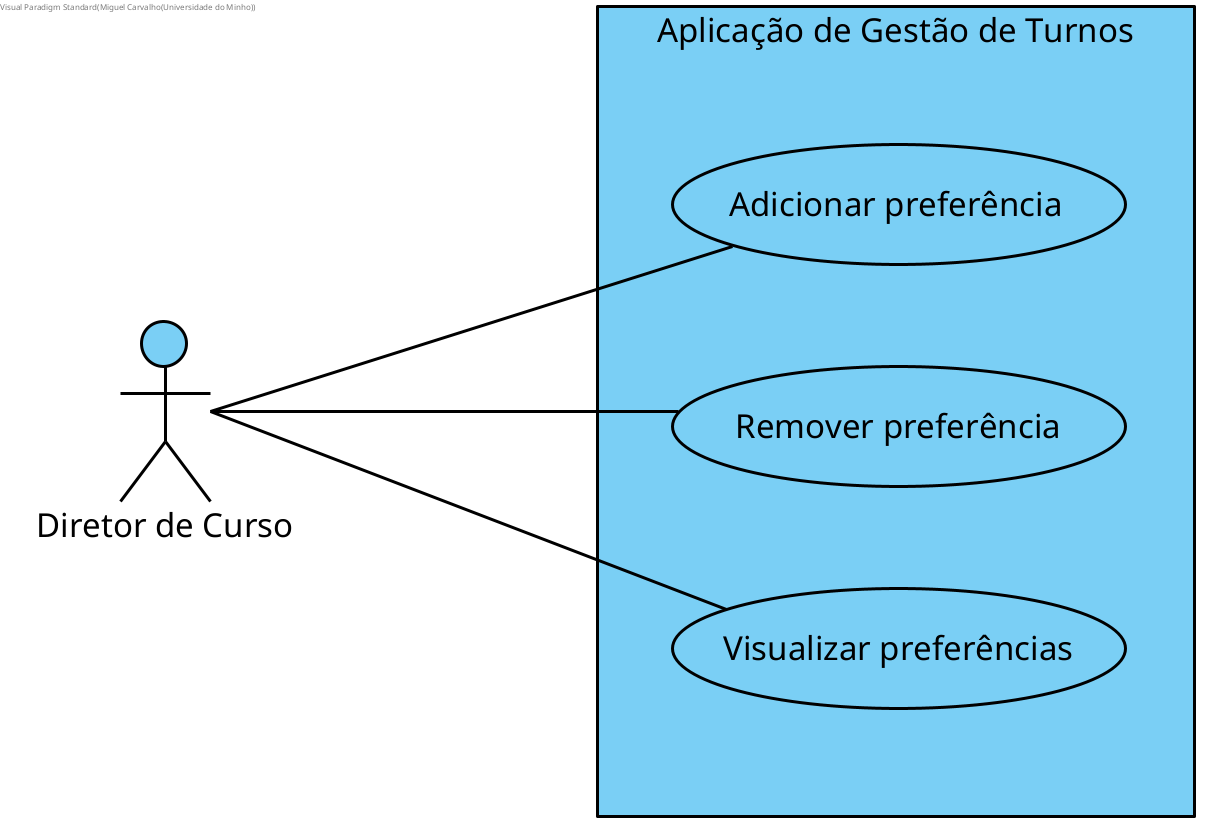
\includegraphics[width=1\textwidth]{images/use-cases/diagrams/3-gestao-preferencias.png}
    \captionof{figure}{Diagrama de Casos de Uso - Gestão de Preferências para UCs}
    \label{fig:2-3-diagrama_de_casos_de_uso_gestao_de_preferencias}
\end{minipage}

\vspace{1cm}

\begin{minipage}{\textwidth}
    \centering
    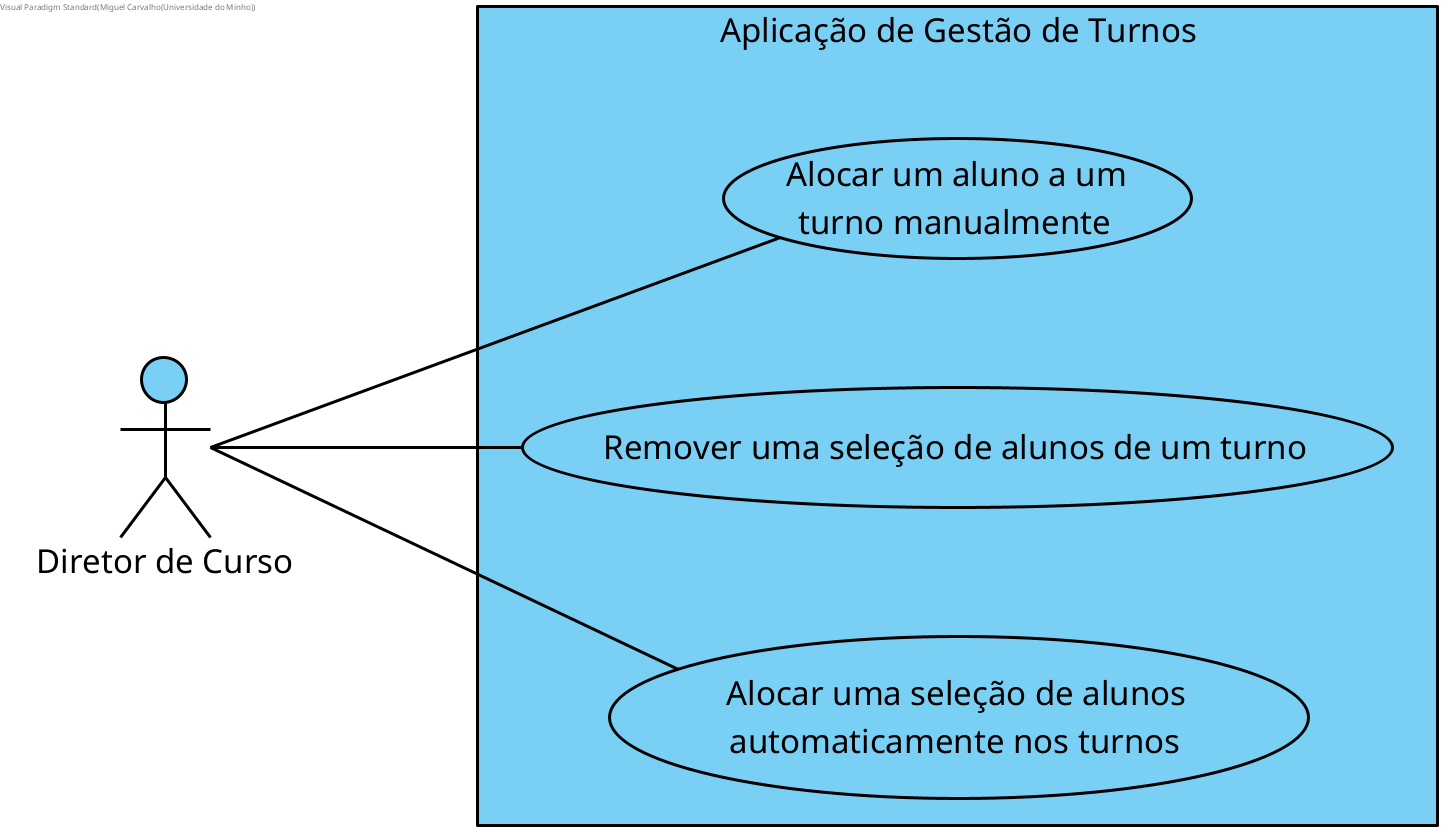
\includegraphics[width=1\textwidth]{images/use-cases/diagrams/4-alocacao-alunos.png}
    \captionof{figure}{Diagrama de Casos de Uso - Alocação de Alunos a Turnos}
    \label{fig:2-4-diagrama_de_casos_de_uso_alocacao_de_alunos}
\end{minipage}

%==========================================================================
% END DIAGRAMAS DE CASOS DE USO
%==========================================================================

%==========================================================================
% BEGIN ESPECIFICAÇÕES DE CASOS DE USO
%==========================================================================

\chapter{Especificações de Casos de Uso}
\vspace{1cm}

% 01-Instalar aplicação.png
\begin{minipage}{\textwidth}
    \centering
    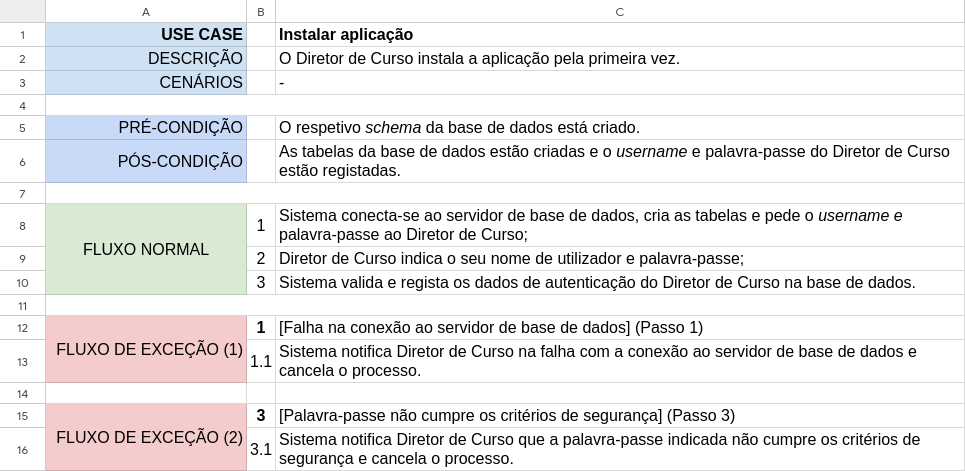
\includegraphics[width=1\textwidth]{images/use-cases/descriptions/01-Instalar aplicação.png}
    \captionof{figure}{\textit{Use Case} Instalar aplicação}
    \label{fig:3-01-instalar_aplicacao}
\end{minipage}

% 02-Autenticação.png
\begin{minipage}{\textwidth}
    \centering
    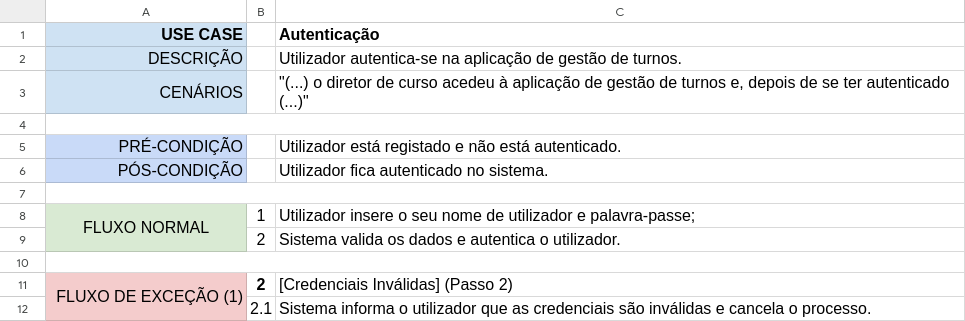
\includegraphics[width=1\textwidth]{images/use-cases/descriptions/02-Autenticação.png}
    \captionof{figure}{\textit{Use Case} Autenticação}
    \label{fig:3-02-autenticacao}
\end{minipage}

% 03-Desautenticação.png
\begin{minipage}{\textwidth}
    \centering
    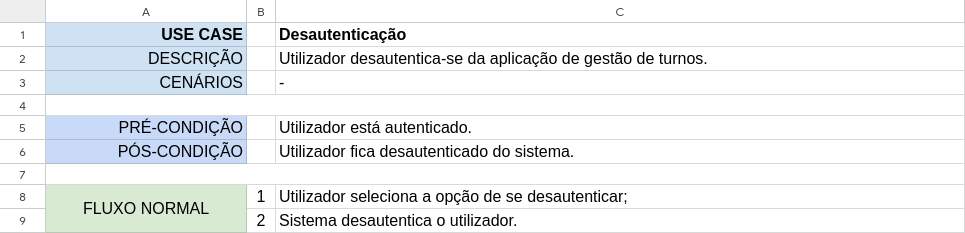
\includegraphics[width=1\textwidth]{images/use-cases/descriptions/03-Desautenticação.png}
    \captionof{figure}{\textit{Use Case} Desautenticação}
    \label{fig:3-03-desautenticacao}
\end{minipage}

% 04-Visualizar Horário.png
\begin{minipage}{\textwidth}
    \centering
    \includegraphics[width=1\textwidth]{images/use-cases/descriptions/04-Visualizar Horário.png}
    \captionof{figure}{\textit{Use Case} Visualizar Horário}
    \label{fig:3-04-visualizar_horario}
\end{minipage}

% 05-Exportar Horário.png
\begin{minipage}{\textwidth}
    \centering
    \includegraphics[width=1\textwidth]{images/use-cases/descriptions/05-Exportar Horário.png}
    \captionof{figure}{\textit{Use Case} Exportar Horário}
    \label{fig:3-05-exportar_horario}
\end{minipage}

% 06-Publicar horários de uma seleção de alunos.png
\begin{minipage}{\textwidth}
    \centering
    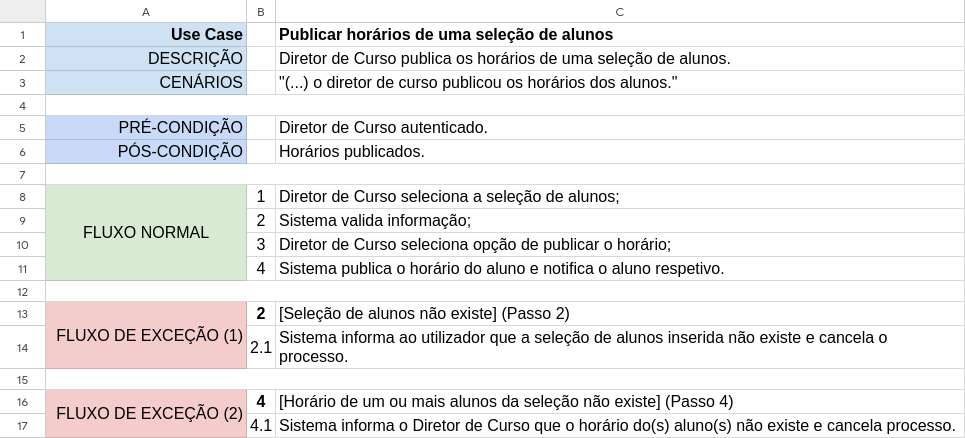
\includegraphics[width=1\textwidth]{images/use-cases/descriptions/06-Publicar horários de uma seleção de alunos.png}
    \captionof{figure}{\textit{Use Case} Publicar horários de uma seleção de alunos}
    \label{fig:3-06-publicar_horarios_de_uma_selecao_de_alunos}
\end{minipage}

% 07-Importar alunos.png
\begin{minipage}{\textwidth}
    \centering
    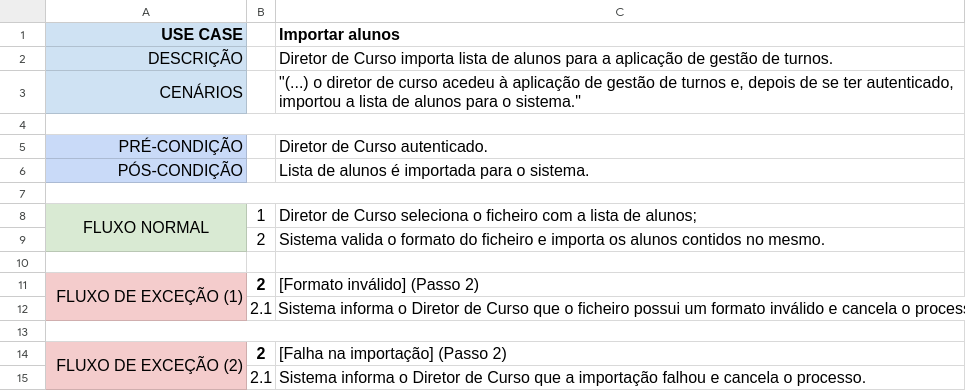
\includegraphics[width=1\textwidth]{images/use-cases/descriptions/07-Importar alunos.png}
    \captionof{figure}{\textit{Use Case} Importar alunos}
    \label{fig:3-07-importar_alunos}
\end{minipage}

% 08-Adicionar aluno.png
\begin{minipage}{\textwidth}
    \centering
    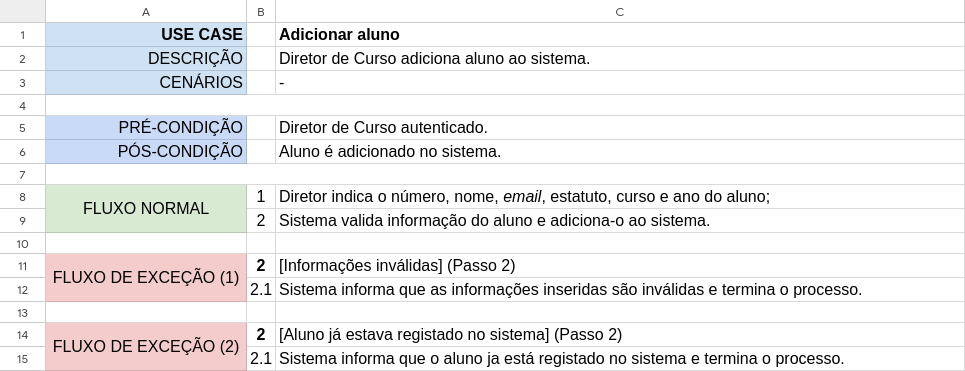
\includegraphics[width=1\textwidth]{images/use-cases/descriptions/08-Adicionar aluno.png}
    \captionof{figure}{\textit{Use Case} Adicionar aluno}
    \label{fig:3-08-adicionar_aluno}
\end{minipage}

% 09-Remover uma seleção de alunos.png
\begin{minipage}{\textwidth}
    \centering
    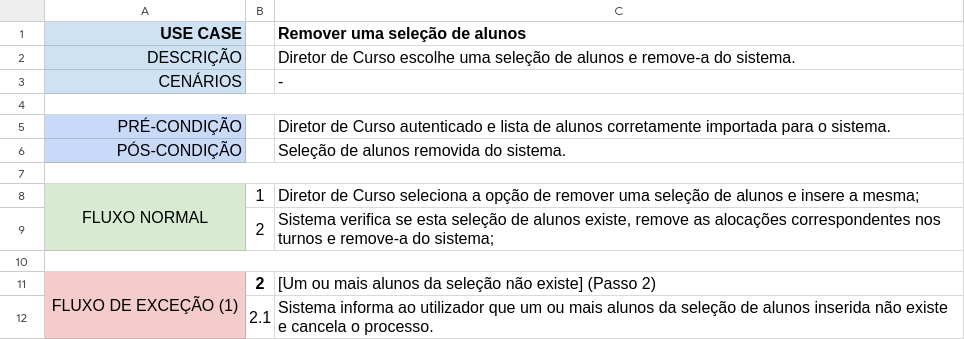
\includegraphics[width=1\textwidth]{images/use-cases/descriptions/09-Remover uma seleção de alunos.png}
    \captionof{figure}{\textit{Use Case} Remover uma seleção de alunos}
    \label{fig:3-09-remover_uma_selecao_de_alunos}
\end{minipage}

% 10-Editar aluno.png
\begin{minipage}{\textwidth}
    \centering
    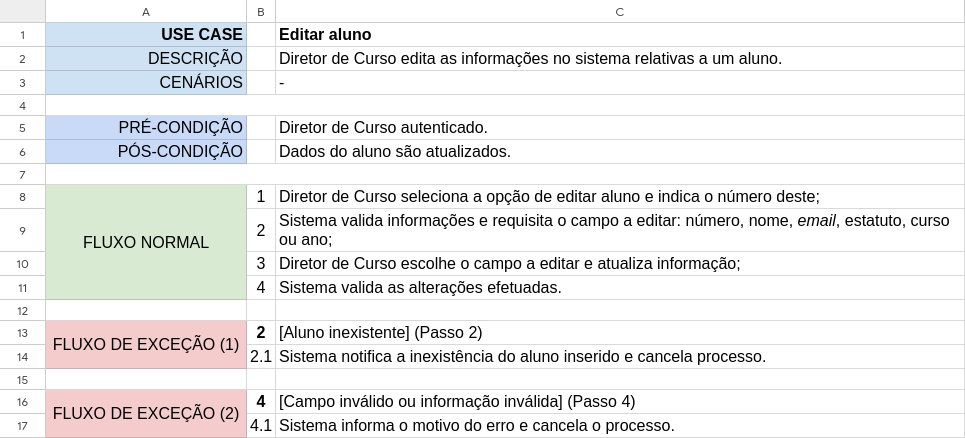
\includegraphics[width=1\textwidth]{images/use-cases/descriptions/10-Editar aluno.png}
    \captionof{figure}{\textit{Use Case} Editar aluno}
    \label{fig:3-10-editar_aluno}
\end{minipage}

% 11-Importar UCs.png
\begin{minipage}{\textwidth}
    \centering
    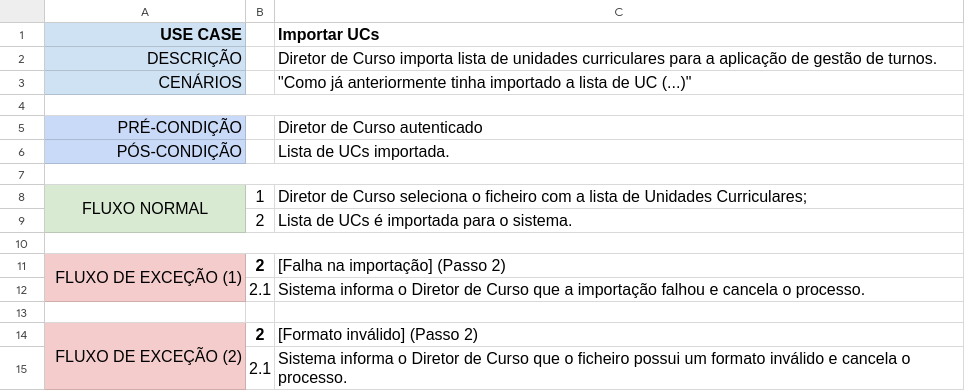
\includegraphics[width=1\textwidth]{images/use-cases/descriptions/11-Importar UCs.png}
    \captionof{figure}{\textit{Use Case} Importar UCs}
    \label{fig:3-11-importar_ucs}
\end{minipage}

% 12-Adicionar UC.png
\begin{minipage}{\textwidth}
    \centering
    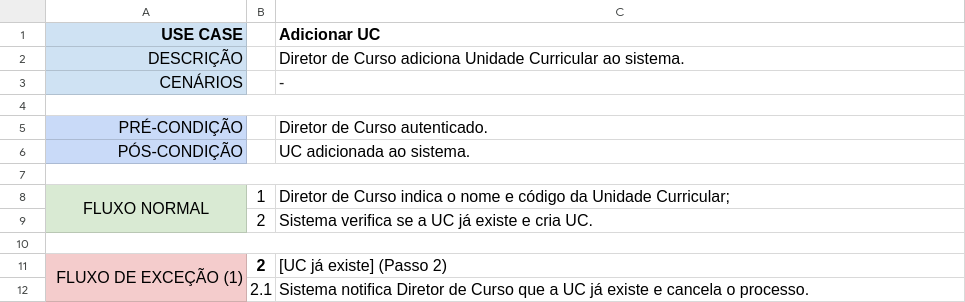
\includegraphics[width=1\textwidth]{images/use-cases/descriptions/12-Adicionar UC.png}
    \captionof{figure}{\textit{Use Case} Adicionar UC}
    \label{fig:3-12-adicionar_uc}
\end{minipage}

% 13-Remover UC.png
\begin{minipage}{\textwidth}
    \centering
    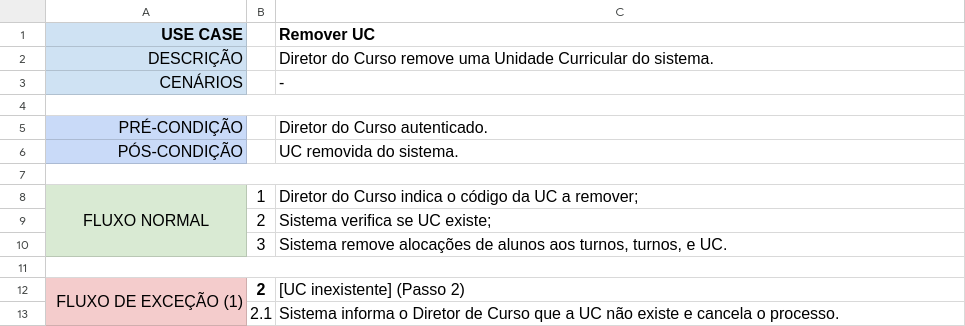
\includegraphics[width=1\textwidth]{images/use-cases/descriptions/13-Remover UC.png}
    \captionof{figure}{\textit{Use Case} Remover UC}
    \label{fig:3-13-remover_uc}
\end{minipage}

% 14-Editar UC.png
\begin{minipage}{\textwidth}
    \centering
    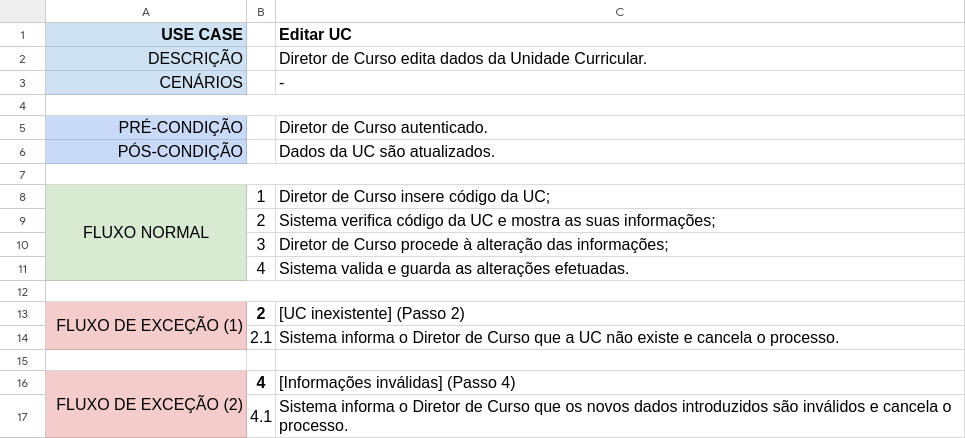
\includegraphics[width=1\textwidth]{images/use-cases/descriptions/14-Editar UC.png}
    \captionof{figure}{\textit{Use Case} Editar UC}
    \label{fig:3-14-editar_uc}
\end{minipage}

% 15-Importar salas.png
\begin{minipage}{\textwidth}
    \centering
    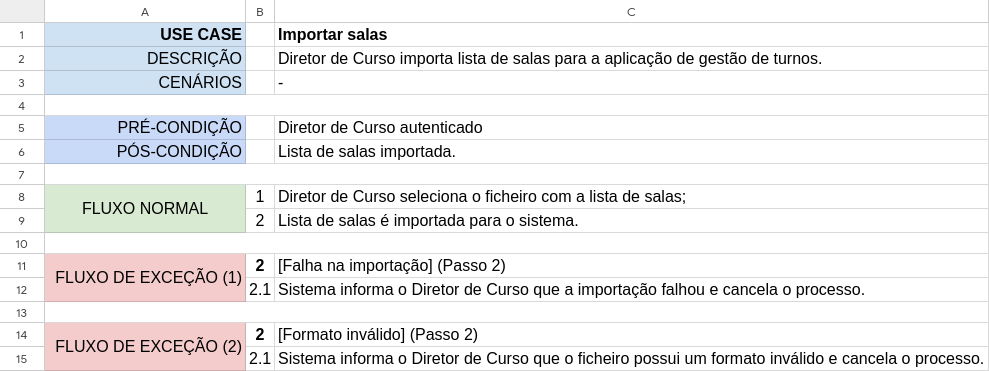
\includegraphics[width=1\textwidth]{images/use-cases/descriptions/15-Importar salas.png}
    \captionof{figure}{\textit{Use Case} Importar salas}
    \label{fig:3-15-importar_salas}
\end{minipage}

% 16-Adicionar sala.png
\begin{minipage}{\textwidth}
    \centering
    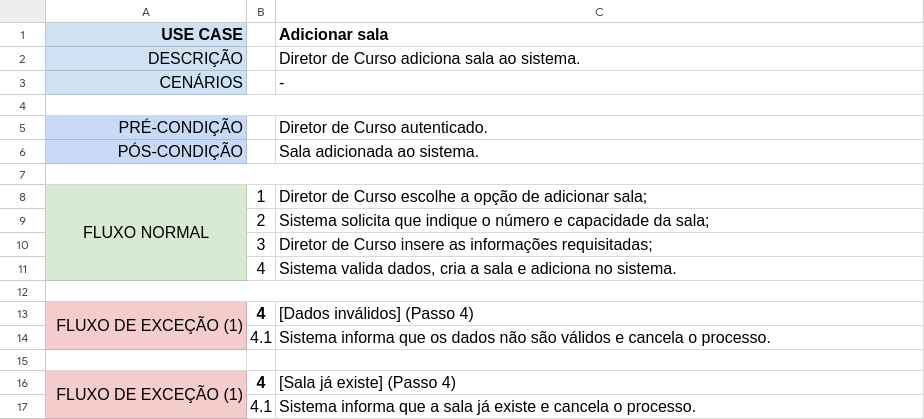
\includegraphics[width=1\textwidth]{images/use-cases/descriptions/16-Adicionar sala.png}
    \captionof{figure}{\textit{Use Case} Adicionar sala}
    \label{fig:3-16-adicionar_sala}
\end{minipage}

% 17-Remover sala.png
\begin{minipage}{\textwidth}
    \centering
    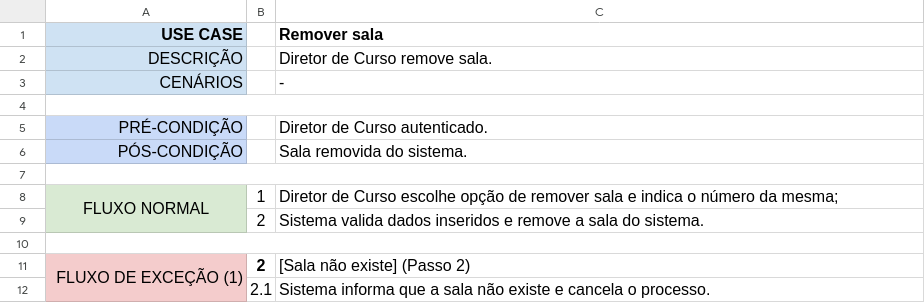
\includegraphics[width=1\textwidth]{images/use-cases/descriptions/17-Remover sala.png}
    \captionof{figure}{\textit{Use Case} Remover sala}
    \label{fig:3-17-remover_sala}
\end{minipage}

% 18-Editar sala.png
\begin{minipage}{\textwidth}
    \centering
    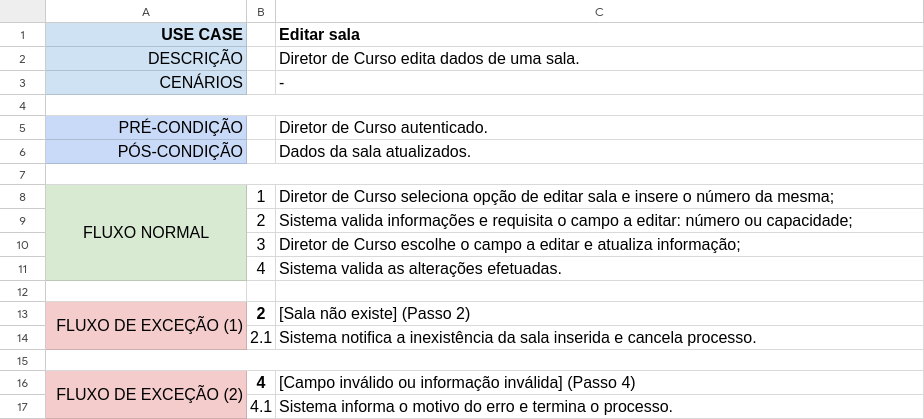
\includegraphics[width=1\textwidth]{images/use-cases/descriptions/18-Editar sala.png}
    \captionof{figure}{\textit{Use Case} Editar sala}
    \label{fig:3-18-editar_sala}
\end{minipage}

% 19-Importar turnos.png
\begin{minipage}{\textwidth}
    \centering
    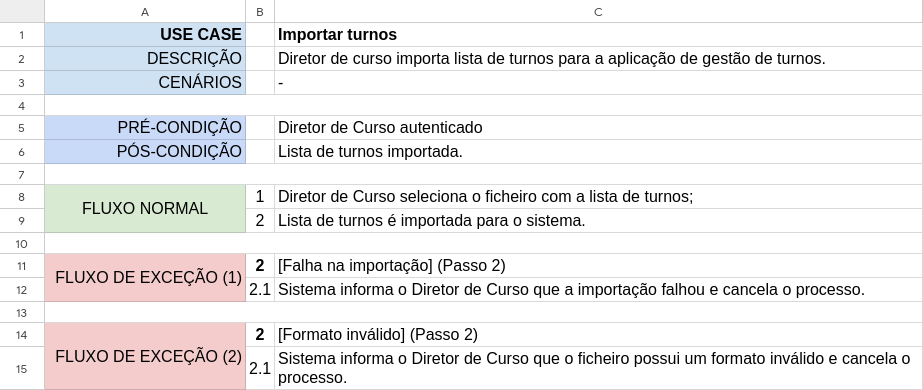
\includegraphics[width=1\textwidth]{images/use-cases/descriptions/19-Importar turnos.png}
    \captionof{figure}{\textit{Use Case} Importar turnos}
    \label{fig:3-19-importar_turnos}
\end{minipage}

% 20-Adicionar turno.png
\begin{minipage}{\textwidth}
    \centering
    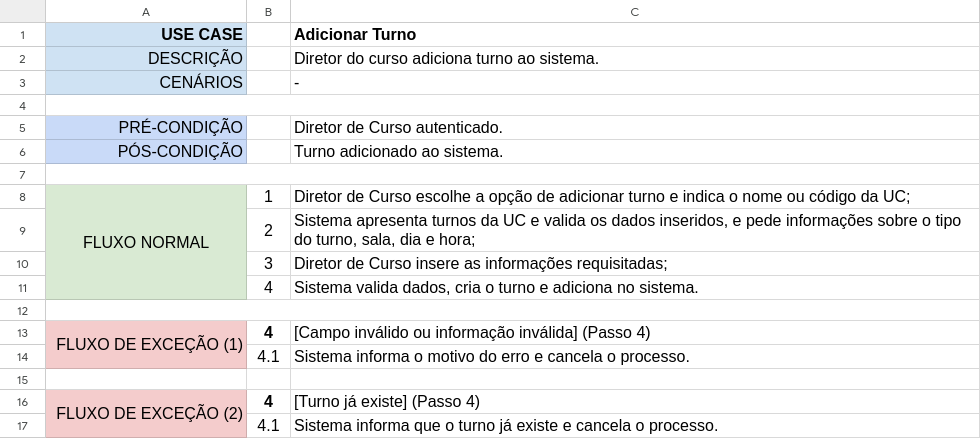
\includegraphics[width=1\textwidth]{images/use-cases/descriptions/20-Adicionar turno.png}
    \captionof{figure}{\textit{Use Case} Adicionar turno}
    \label{fig:3-20-adicionar_turno}
\end{minipage}

% 21-Remover turno.png
\begin{minipage}{\textwidth}
    \centering
    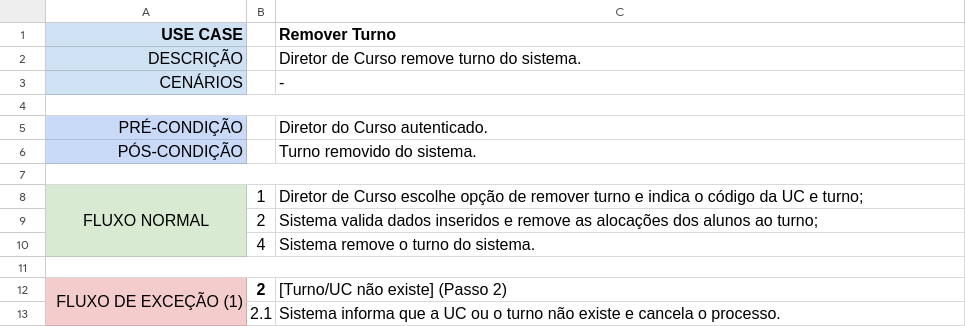
\includegraphics[width=1\textwidth]{images/use-cases/descriptions/21-Remover turno.png}
    \captionof{figure}{\textit{Use Case} Remover turno}
    \label{fig:3-21-remover_turno}
\end{minipage}

% 22-Editar turno.png
\begin{minipage}{\textwidth}
    \centering
    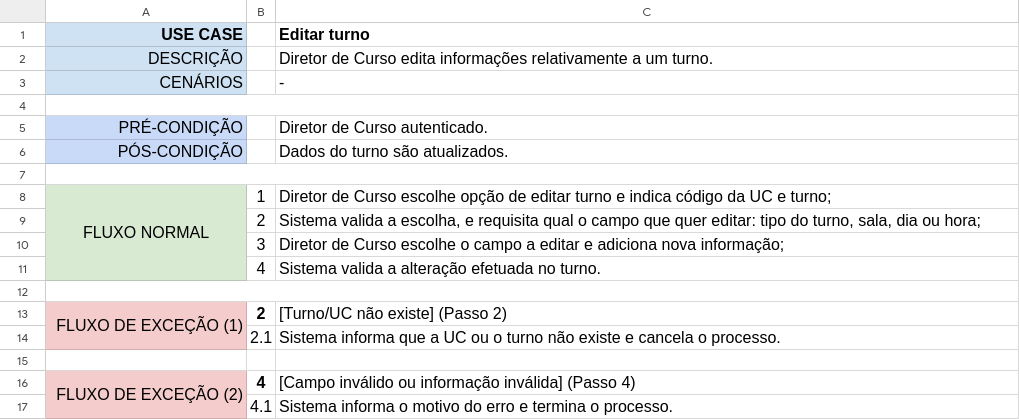
\includegraphics[width=1\textwidth]{images/use-cases/descriptions/22-Editar turno.png}
    \captionof{figure}{\textit{Use Case} Editar turno}
    \label{fig:3-22-editar_turno}
\end{minipage}

% 23-Importar Cursos.png
\begin{minipage}{\textwidth}
    \centering
    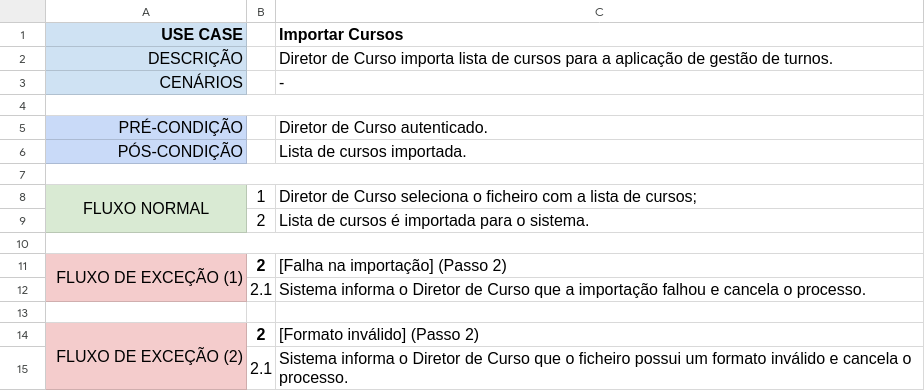
\includegraphics[width=1\textwidth]{images/use-cases/descriptions/23-Importar Cursos.png}
    \captionof{figure}{\textit{Use Case} Importar Cursos}
    \label{fig:3-23-importar_cursos}
\end{minipage}

% 24-Adicionar Curso.png
\begin{minipage}{\textwidth}
    \centering
    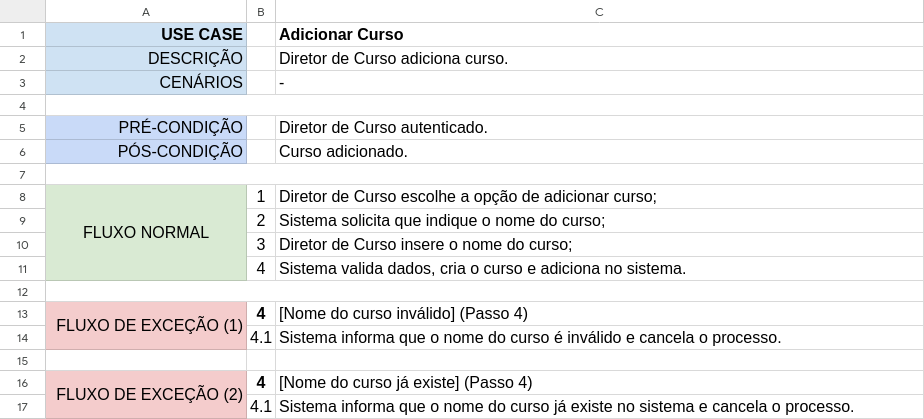
\includegraphics[width=1\textwidth]{images/use-cases/descriptions/24-Adicionar Curso.png}
    \captionof{figure}{\textit{Use Case} Adicionar Curso}
    \label{fig:3-24-adicionar_curso}
\end{minipage}

% 25-Remover Curso.png
\begin{minipage}{\textwidth}
    \centering
    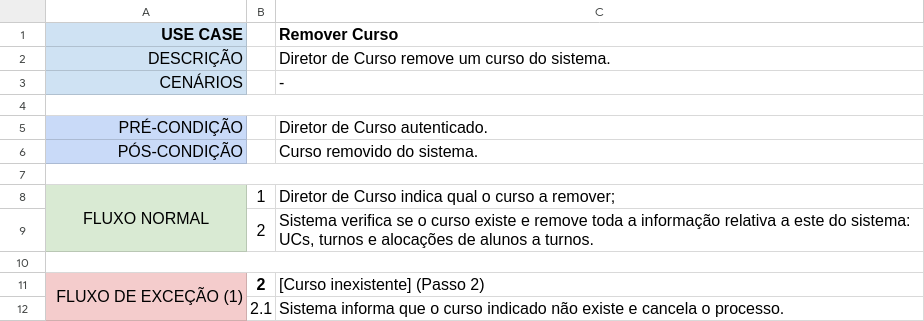
\includegraphics[width=1\textwidth]{images/use-cases/descriptions/25-Remover Curso.png}
    \captionof{figure}{\textit{Use Case} Remover Curso}
    \label{fig:3-25-remover_curso}
\end{minipage}

% 26-Editar Curso.png
\begin{minipage}{\textwidth}
    \centering
    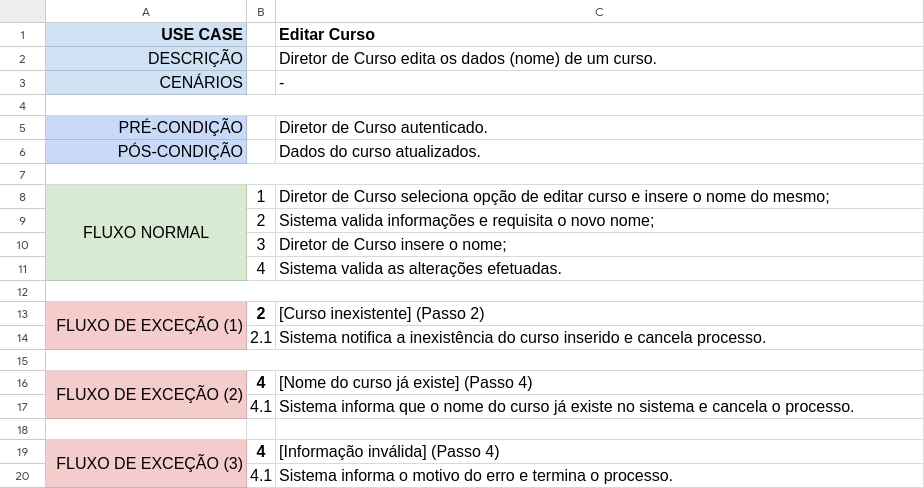
\includegraphics[width=1\textwidth]{images/use-cases/descriptions/26-Editar Curso.png}
    \captionof{figure}{\textit{Use Case} Editar Curso}
    \label{fig:3-26-editar_curso}
\end{minipage}

% 27-Adicionar preferência.png
\begin{minipage}{\textwidth}
    \centering
    \includegraphics[width=1\textwidth]{images/use-cases/descriptions/27-Adicionar preferência.png}
    \captionof{figure}{\textit{Use Case} Adicionar preferência}
    \label{fig:3-27-adicionar_preferencia}
\end{minipage}

% 28-Remover preferência.png
\begin{minipage}{\textwidth}
    \centering
    \includegraphics[width=1\textwidth]{images/use-cases/descriptions/28-Remover preferência.png}
    \captionof{figure}{\textit{Use Case} Remover preferência}
    \label{fig:3-28-remover_preferencia}
\end{minipage}

% 29-Visualizar preferências.png
\begin{minipage}{\textwidth}
    \centering
    \includegraphics[width=1\textwidth]{images/use-cases/descriptions/29-Visualizar preferências.png}
    \captionof{figure}{\textit{Use Case} Visualizar preferências}
    \label{fig:3-29-visualizar_preferencias}
\end{minipage}

% 30-Alocar um aluno a um turno manualmente.png
\begin{minipage}{\textwidth}
    \centering
    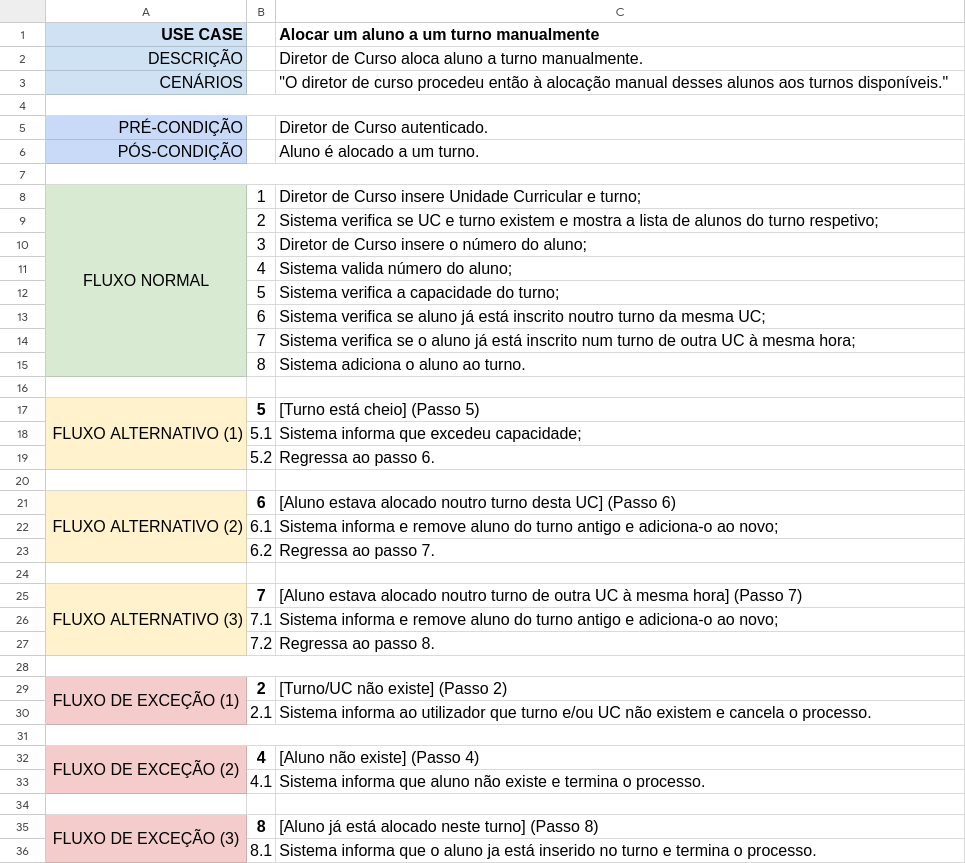
\includegraphics[width=1\textwidth]{images/use-cases/descriptions/30-Alocar um aluno a um turno manualmente.png}
    \captionof{figure}{\textit{Use Case} Alocar um aluno a um turno manualmente}
    \label{fig:3-30-alocar_um_aluno_a_um_turno_manualmente}
\end{minipage}

% 31-Alocar uma seleção de alunos automaticamente nos turnos.png
\begin{minipage}{\textwidth}
    \centering
    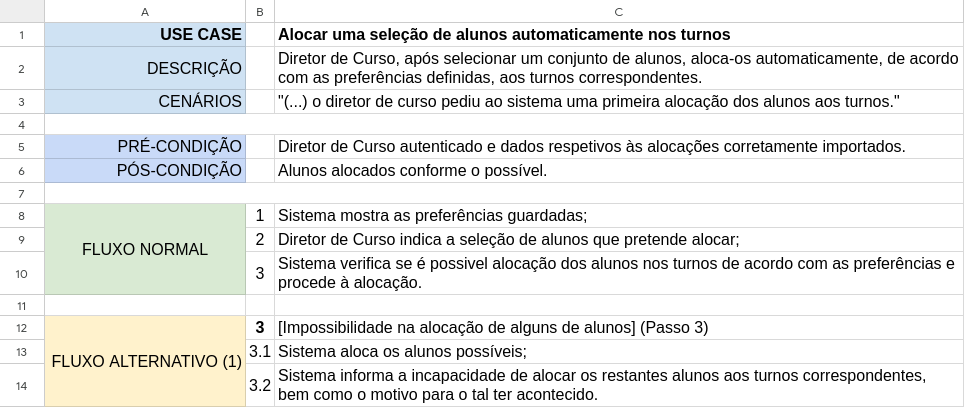
\includegraphics[width=1\textwidth]{images/use-cases/descriptions/31-Alocar uma seleção de alunos automaticamente nos turnos.png}
    \captionof{figure}{\textit{Use Case} Alocar uma seleção de alunos automaticamente nos turnos}
    \label{fig:3-31-alocar_uma_selecao_de_alunos_automaticamente_nos_turnos}
\end{minipage}

% 32-Remover uma seleção de alunos de um turno manualmente.png
\begin{minipage}{\textwidth}
    \centering
    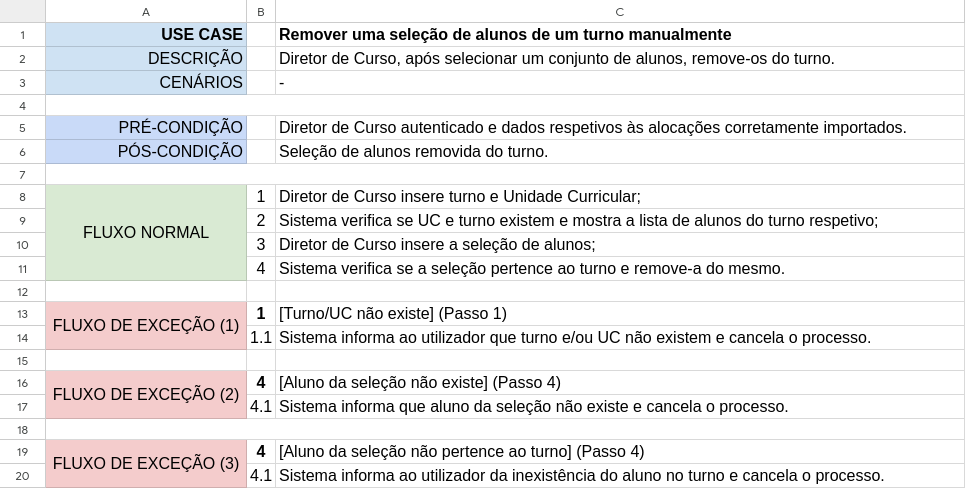
\includegraphics[width=1\textwidth]{images/use-cases/descriptions/32-Remover uma seleção de alunos de um turno manualmente.png}
    \captionof{figure}{\textit{Use Case} Remover uma seleção de alunos de um turno manualmente}
    \label{fig:3-32-remover_uma_selecao_de_alunos_de_um_turno_manualmente}
\end{minipage}

%==========================================================================
% END ESPECIFICAÇÕES DE CASOS DE USO
%==========================================================================

%==========================================================================
% BEGIN CONSIDERAÇÕES PERTINENTES
%==========================================================================

\chapter{Considerações Pertinentes}
\vspace{1cm}

Ao longo dos casos de uso apresentados, foi utilizado o termo “seleção de alunos”.
Este termo refere-se a um conjunto de alunos que foram selecionados com base em critérios específicos,
como por exemplo, alunos de um determinado ano, unidade curricular, com estatuto, entre outros.

Esta generalização permite que os casos de uso sejam mais flexíveis
e possam ser aplicados a diferentes situações. Como por exemplo, a alocação de somente
um aluno, selecionado atráves do seu número, a um turno.

A seleção de alunos também permite ao Diretor de Curso a definição da ordem
a qual os alunos devem ser alocados a turnos.

\vspace{1cm}

Caso a monotorização de atividades, através de um sistema de \textit{logs}, fosse um requisito funcional,
desejado pela equipa docente, seria possível adicionar um caso de uso que permitisse a visualização
de \textit{logs} de atividade, como por exemplo, a data e hora de criação de um turno,
ou a data e hora de alocação de um aluno a um turno. Para tal, seria necessário
incorporar esta ação do sistema nos casos de uso, nos quais se justificaria registar tal ação.

%==========================================================================
% END CONSIDERAÇÕES PERTINENTES
%==========================================================================

%==========================================================================
% BEGIN BIBLIOGRAFIA
%==========================================================================

%% Changes biblibography name
%% Portuguese babel default : “Bibliografia”
%% Personally I prefer “Referências”
% \renewcommand\bibname{Referências}

%% https://www.overleaf.com/learn/latex/bibliography_management_with_bibtex
% \begin{thebibliography}{9}
% \bibitem{DatabaseSystems}
% Connolly, T., \& Begg, C. (2015). Database Systems: A Practical Approach to Design, Implementation, and Management (6th ed.). Pearson Education. London, UK.
%
% \bibitem{Aprendizagem em Banco de Dados}
% Cândido, C. H. (2005). Aprendizagem em Banco de Dados: Implementação de Ferramenta de Modelagem E.R. Monografia de Especialização. Universidade Federal de Santa Catarina, Brasil.
%
% \bibitem{MySQLManual}
% MySQL 8.0 Reference Manual (2024). \href{https://dev.mysql.com/doc/refman/8.0/en/storage-requirements.html}{\underline{MySQL 8.0 Reference Manual: Data Type Storage} \underline{Requirements}}. MySQL, Oracle.
% \end{thebibliography}

%% Add bibliografia to index
% \addcontentsline{toc}{chapter}{Bibliografia}

%==========================================================================
% END BIBLIOGRAFIA
%==========================================================================

%==========================================================================
% BEGIN LISTA DE SIGLAS E ACRÓNIMOS
%==========================================================================

%% Portuguese babel does not translate this environment
\renewcommand{\nomname}{Lista de Siglas e Acrónimos}

%% acronyms
\nomenclature[01]{\textbf{BD}}{Base de Dados}
\nomenclature[02]{\textbf{SBD}}{Sistema de Base de Dados}

%% Show acronyms
% \printnomenclature

%==========================================================================
% END LISTA DE SIGLAS E ACRÓNIMOS
%==========================================================================

%==========================================================================
% BEGIN ANEXOS
%==========================================================================
%
%% Why \addchap, instead of \chapter?
%% \addchap has no numbering but appears in table of contents.
% \addchap{Anexos}
%
%     \addsec{
%         \href{https://docs.google.com/spreadsheets/d/1o4Pl00OfLMH4ukDdvNz3TweH2OxFpA7t8Vd_v-Idx-c/edit?usp=sharing}{\small [I] Diagrama de Gantt}
%         \label{anexo:1}
%     }
%
%     \addsec{
%         \href{https://docs.google.com/spreadsheets/d/1ZYYOut1zsdGr3DZ1JqruOHxCBgM_EFV9JDmxPFWZpiY/edit?usp=sharing}{\small [II] Documentos de Requisitos}
%         \label{anexo:2}
%     }

%==========================================================================
% END ANEXOS
%==========================================================================
\end{document}
